%\begin{frame}{Info about negative weights}
%    \begin{itemize}
%        \item Researching
%    \end{itemize}
%\end{frame}

\begin{frame}{Impact of negative weights on the training}
    \begin{columns}
        \begin{column}{0.5\textwidth}
            \begin{figure}
                \centering
                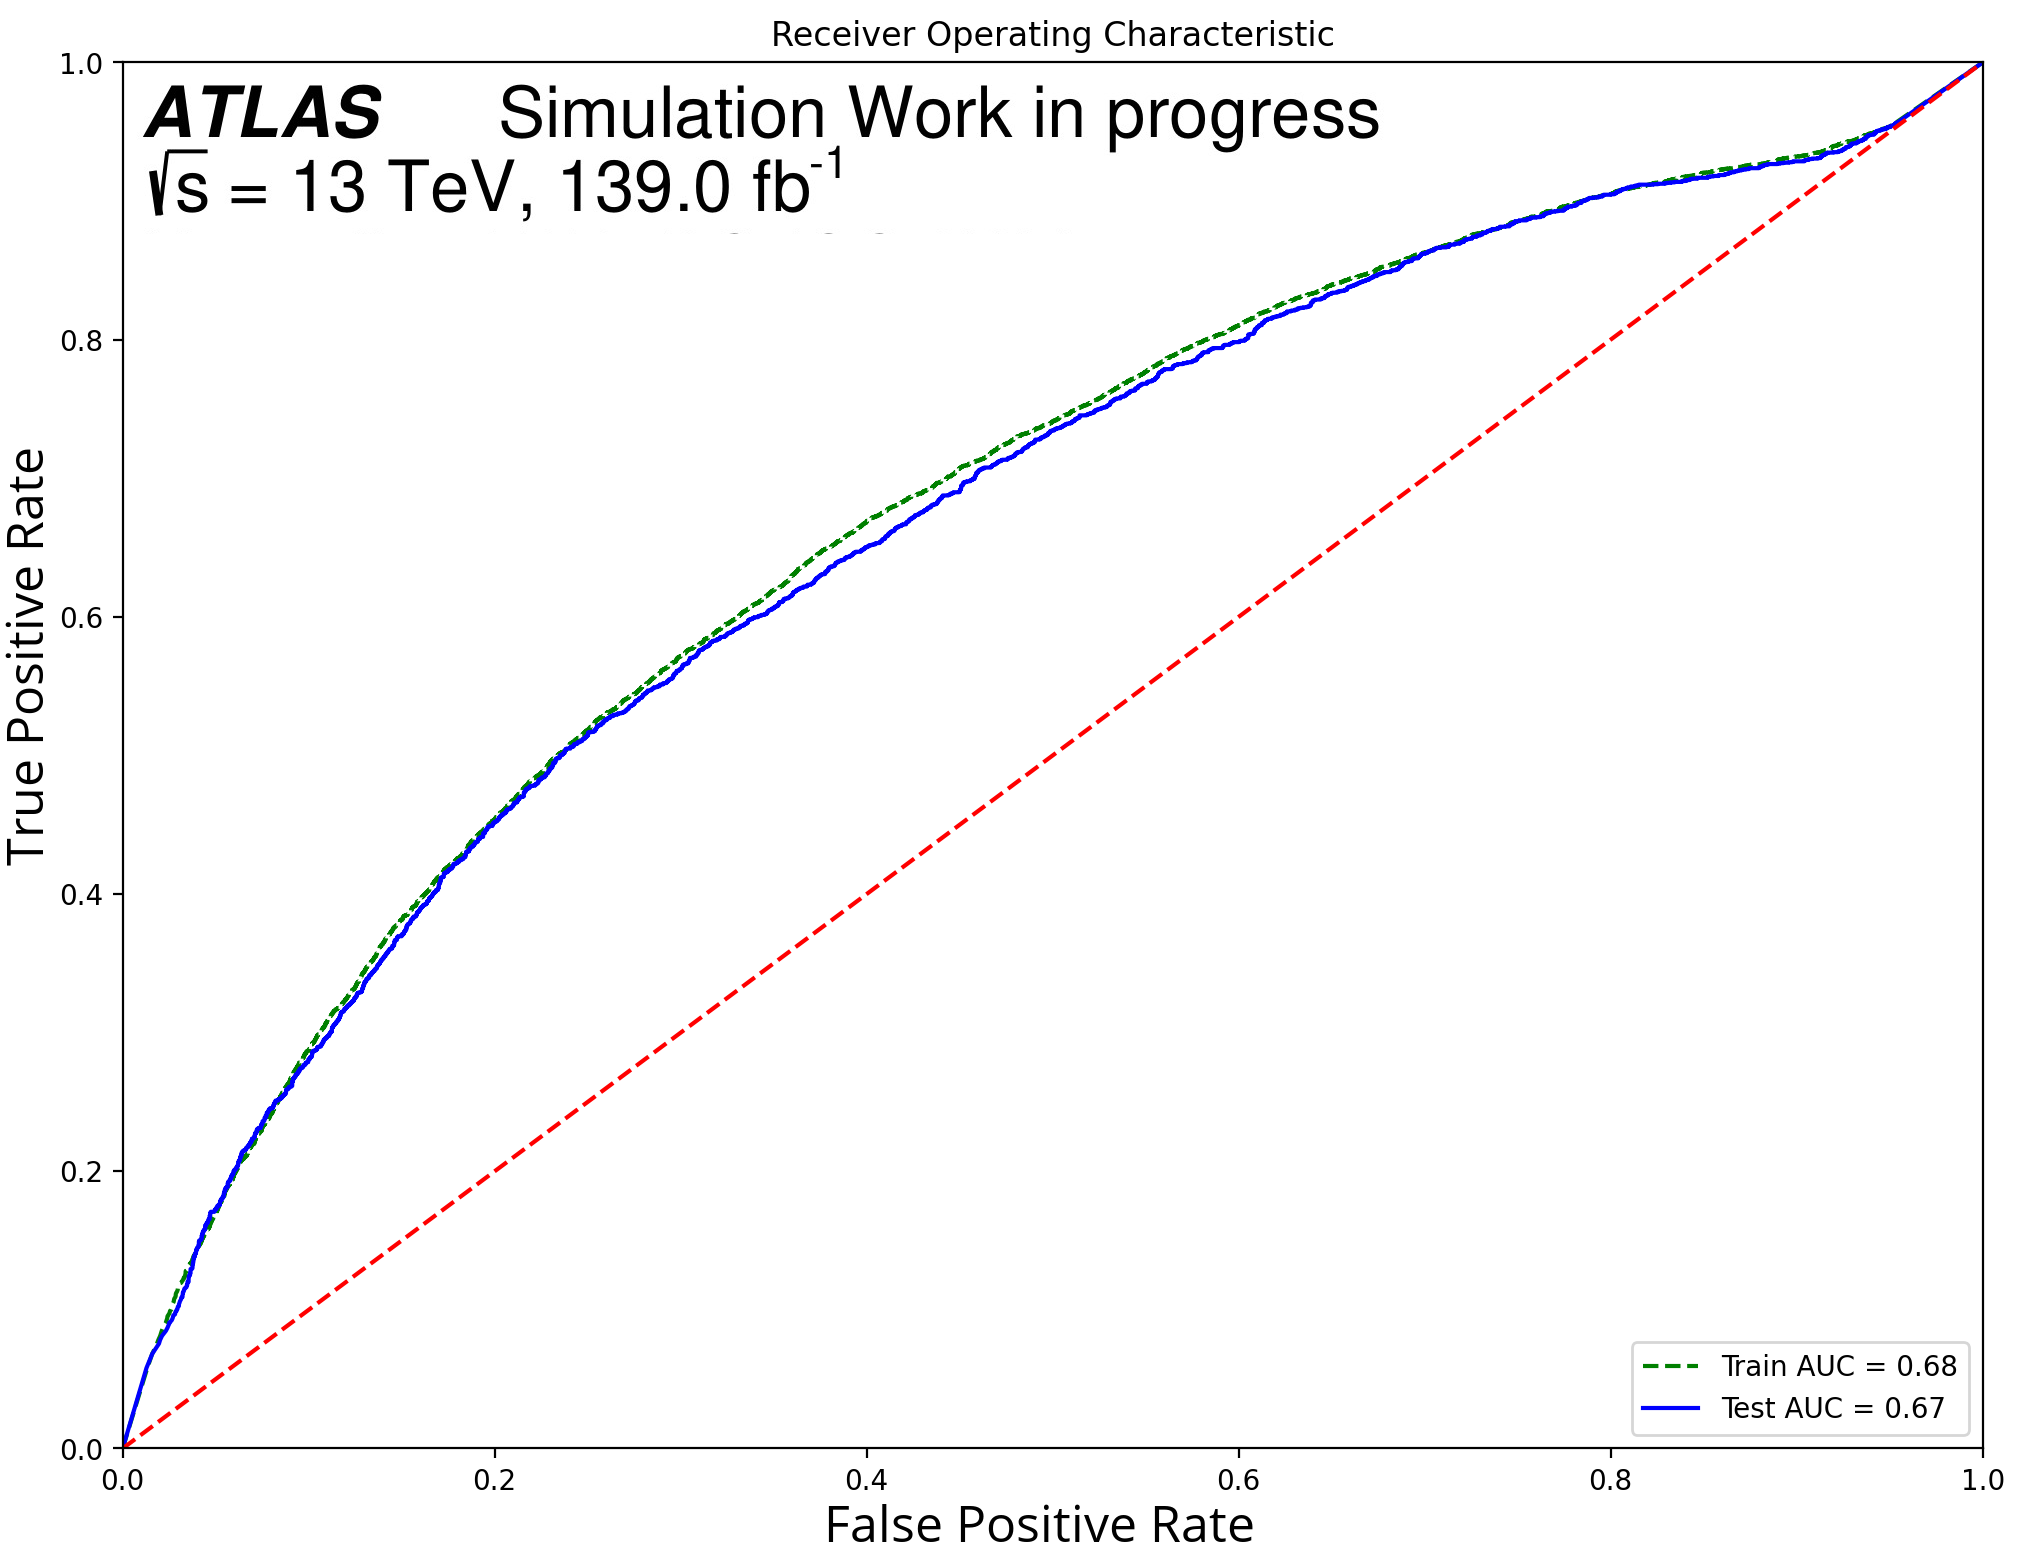
\includegraphics[width=\textwidth]{ROC_normalWeights}
            \end{figure}
        \end{column}
        \begin{column}{0.5\textwidth}
            \begin{figure}
                \centering
                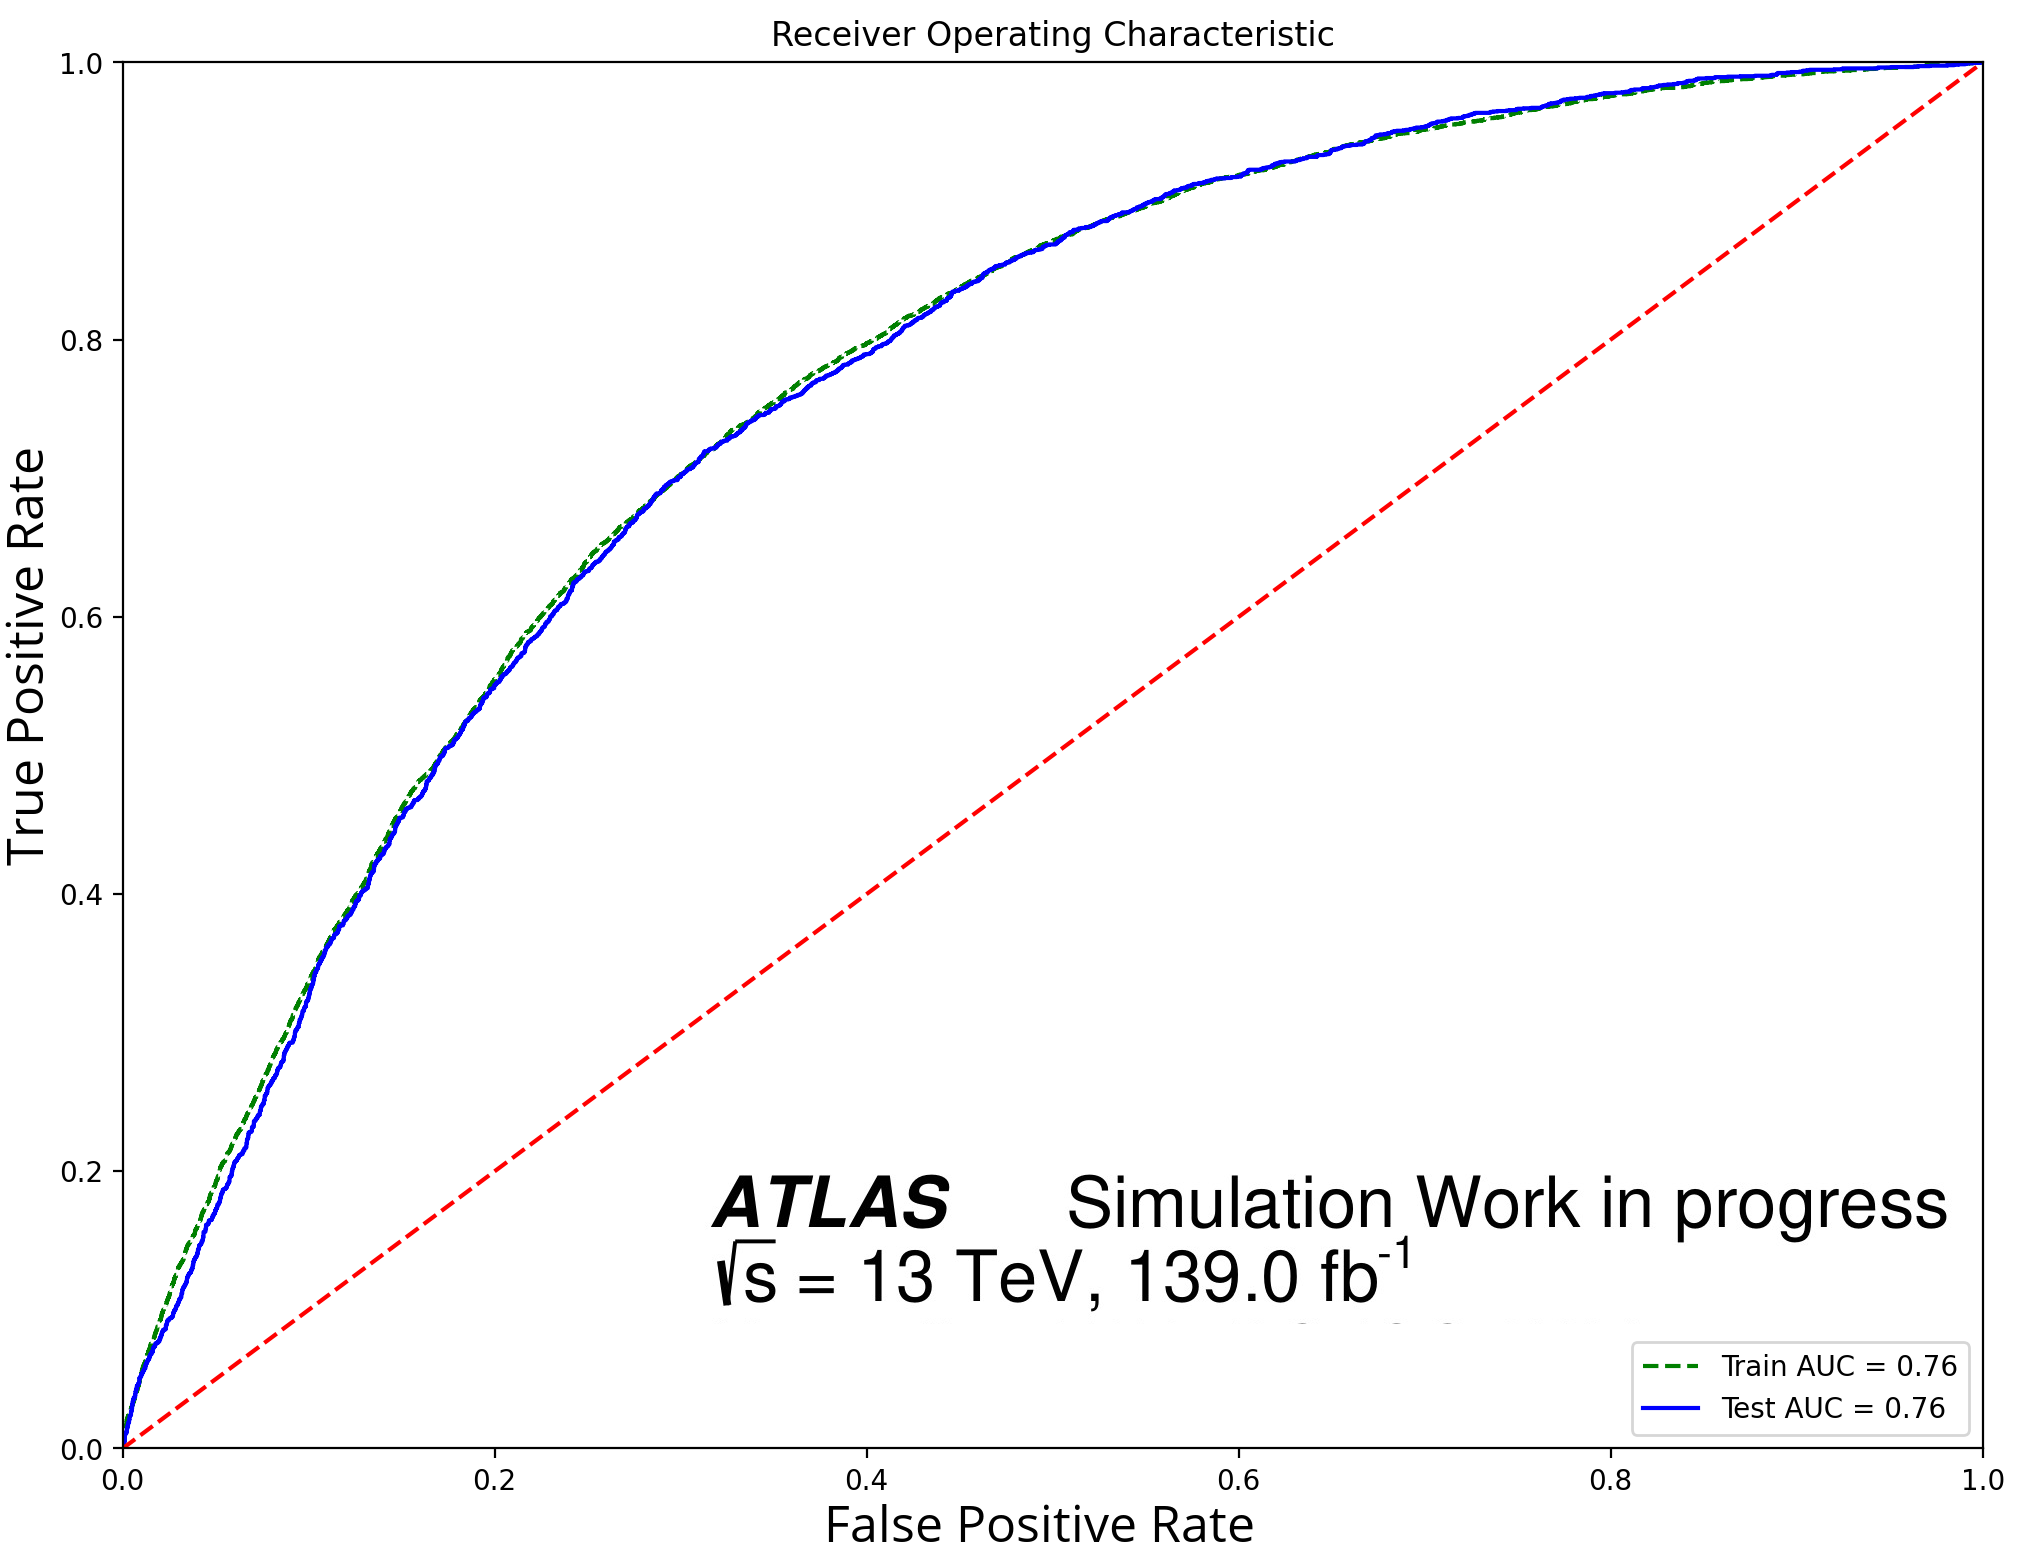
\includegraphics[width=\textwidth]{ROC_absoluteWeights}
            \end{figure}
        \end{column}
    \end{columns}
    \begin{itemize}
        \item About $35 \%$ of events have negative weights
        \item Negative weights break the networks training
        \item Possible ways of handling the weights is to use the absolutes or just use positive weights
    \end{itemize}
\end{frame}